\let\negmedspace\undefined
\let\negthickspace\undefined
\documentclass[journal]{IEEEtran}


\setlength{\headheight}{1cm} % Set the height of the header box
\setlength{\headsep}{0mm}     % Set the distance between the header box and the top of the text
 \usepackage[a4paper,margin=10mm, onecolumn]{geometry}
\usepackage{gvv-book}
\usepackage{gvv}
\usepackage{cite}
\usepackage{amsmath,amssymb,amsfonts,amsthm}
\usepackage{algorithmic}
\usepackage{graphicx}
\usepackage{textcomp}
\usepackage{xcolor}
\usepackage{txfonts}
\usepackage{listings}
\usepackage{enumitem}
\usepackage{mathtools}
\usepackage{gensymb}
\usepackage{comment}
\usepackage[breaklinks=true]{hyperref}
\usepackage{tkz-euclide} 
\usepackage{listings}                                       
\def\inputGnumericTable{}                                
\usepackage[latin1]{inputenc}                                
\usepackage{color}                                            
\usepackage{array}                                            
\usepackage{longtable}                                       
\usepackage{calc}                                             
\usepackage{multirow}                                         
\usepackage{hhline}                                           
\usepackage{ifthen}                                           
\usepackage{lscape}
\usepackage{circuitikz}
\tikzstyle{block} = [rectangle, draw, fill=blue!20, 
    text width=4em, text centered, rounded corners, minimum height=3em]
\tikzstyle{sum} = [draw, fill=blue!10, circle, minimum size=1cm, node distance=1.5cm]
\tikzstyle{input} = [coordinate]
\tikzstyle{output} = [coordinate]

\begin{document}

\bibliographystyle{IEEEtran}
\vspace{3cm}

\title{1.2.19}
\author{AI25BTECH11013-Gautham}
 \maketitle
% \newpage
% \bigskip
{\let\newpage\relax\maketitle}

\renewcommand{\thefigure}{\theenumi}
\renewcommand{\thetable}{\theenumi}
\setlength{\intextsep}{10pt} % Space between text and floats


\numberwithin{equation}{enumi}
\numberwithin{figure}{enumi}
\renewcommand{\thetable}{\theenumi}                          
\textbf{Question}:\\
In which quadrant or on which axis do each of the points $\brak{-2,4},\brak{3,-1},\brak{-1,0},\brak{1,2}$ and $\brak{-3,-5}$ lie?       Verify your answer by locating them on the Cartesian plane?\\
\solution \\
If x=0 then the point $\brak{x,y}$ lies on y-axis.\\
If y=0 then the point $\brak{x,y}$ lies on x-axis.\\
If $x>0,y>0$ then the point $\brak{x,y}$ lies in $1^\text{st}$ quadrant.\\
If $x<0,y>0$ then the point $\brak{x,y}$ lies in $2^\text{nd}$ quadrant. \\
If $x<0,y<0$ then the point $\brak{x,y}$ lies in $3^\text{rd}$ quadrant. \\
If $x>0,y<0$ then the point $\brak{x,y}$ lies in $4^\text{th}$ quadrant. \\
We can infer that $\brak{-2,4}$ lies in $2^\text{nd}$ quadrant as . \\
Similarly $\brak{3,-1}$,$\brak{-1,0}$,$\brak{1,2}$,$\brak{-3,-5}$ lie on $4^\text{th}$quadrant,x-axis,$1^\text{st}$ quadrant,$3^\text{rd}$ quadrant respectively . \\
This can also be verified from the graph below ,
\begin{figure}[h!]
    \centering
    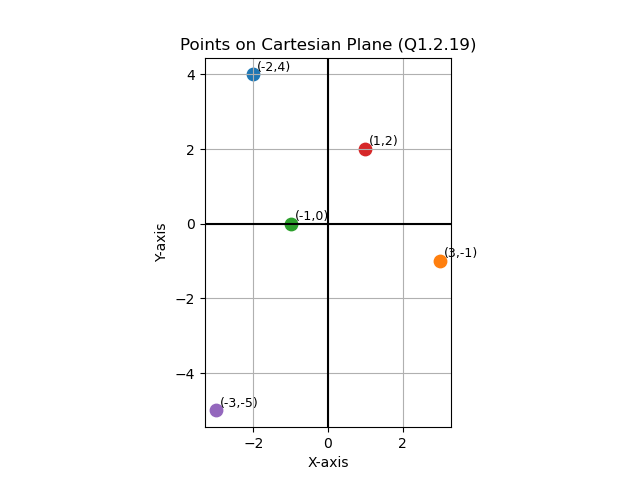
\includegraphics[height=0.6\textheight, keepaspectratio]{figs/Figure1.png}
    \label{figure_1}
\end{figure}

\end{document}
